\documentclass[a4paper]{article}

\usepackage[english]{babel}
\usepackage[utf8]{inputenc}
\usepackage{amsmath,amssymb}
\usepackage{graphicx}
\usepackage[font={small,it}]{caption}
\usepackage[colorinlistoftodos]{todonotes}
\usepackage{placeins}


% Använd dessa om ni vill lägga in kommentarer med \dittnamn{kommentar}
%\newcommand{\robert}[1]{\todo[color=green!40]{#1}}
%\newcommand{\yue}[1]{\todo[color=blue!40]{#1}}
%\newcommand{\martin}[1]{\todo[color=red!40]{#1}}
%\setlength{\marginparwidth}{3cm}
\oddsidemargin=0in
\evensidemargin=0in
\textwidth=6.25in
\headsep=0pt
\headheight=0pt
\topmargin=0in
\textheight=9.5in

\title{Superconductivity}

% Skriv dit ditt namn.
\author{Robert Vedin \\ Yue Jiao \\ Martin Sundin}

\date{April 21, 2016}

\begin{document}
\maketitle

%\begin{abstract}
%Your abstract.
%\end{abstract}


\section{Introduction}

A superconductor is a material whose electrical resistance drops to zero below a certain critical temperature. These materials will also act as a perfect diamagnet such that the magnetic field $\mathbf{B} = 0$ in its interior. These materials can be separated into two sub-groups, type I and type II superconductors, depending on how they react when subject to a sufficiently strong magnetic field.

The type I superconductor material will not allow any magnetic flux within its interior so long as the magnitude of the field stay below some critical value $H_c$, once this critical value is reached the material will lose its superconducting properties.

The type II superconductor material will also prevent any magnetic fields from penetrating the material so long as the magnitude is below the critical value $H_{c1}$. When the applied field has a magnitude greater than $H_{c1}$ the material will enter a vortex state and magnetic field lines will start to penetrate parts of the material. Once the applied field reaches a magnitude $H_{c2}$ the material will completely loose its superconducting properties.

\section{Experimental procedure}
The measurement setup is shown in Figure \ref{setup}, the measurement of the resistance was done by measuring the voltage between points (2) and (3) in a so called four-point measurement. This technique was used in order to get a higher accuracy in the measurement as it will not be influenced by the voltage drop at the contacts (1) and (4).

During the experiment, we first start the measurement software 'cassy lab' and start the measurements. Then the measurement module which is showed in Figure \ref{setup} is put into a box. Then we put enough liquid nitrogen into the container so the whole measurement module is coverd by it. Then we waited resistance of the measurement module showed within the 'cassy lab' dropped to around $0$ and let it stay at $0$ for a short while. Then we took it out and waited the temperature and the resistance returned to original values. 

\begin{figure}
\centering
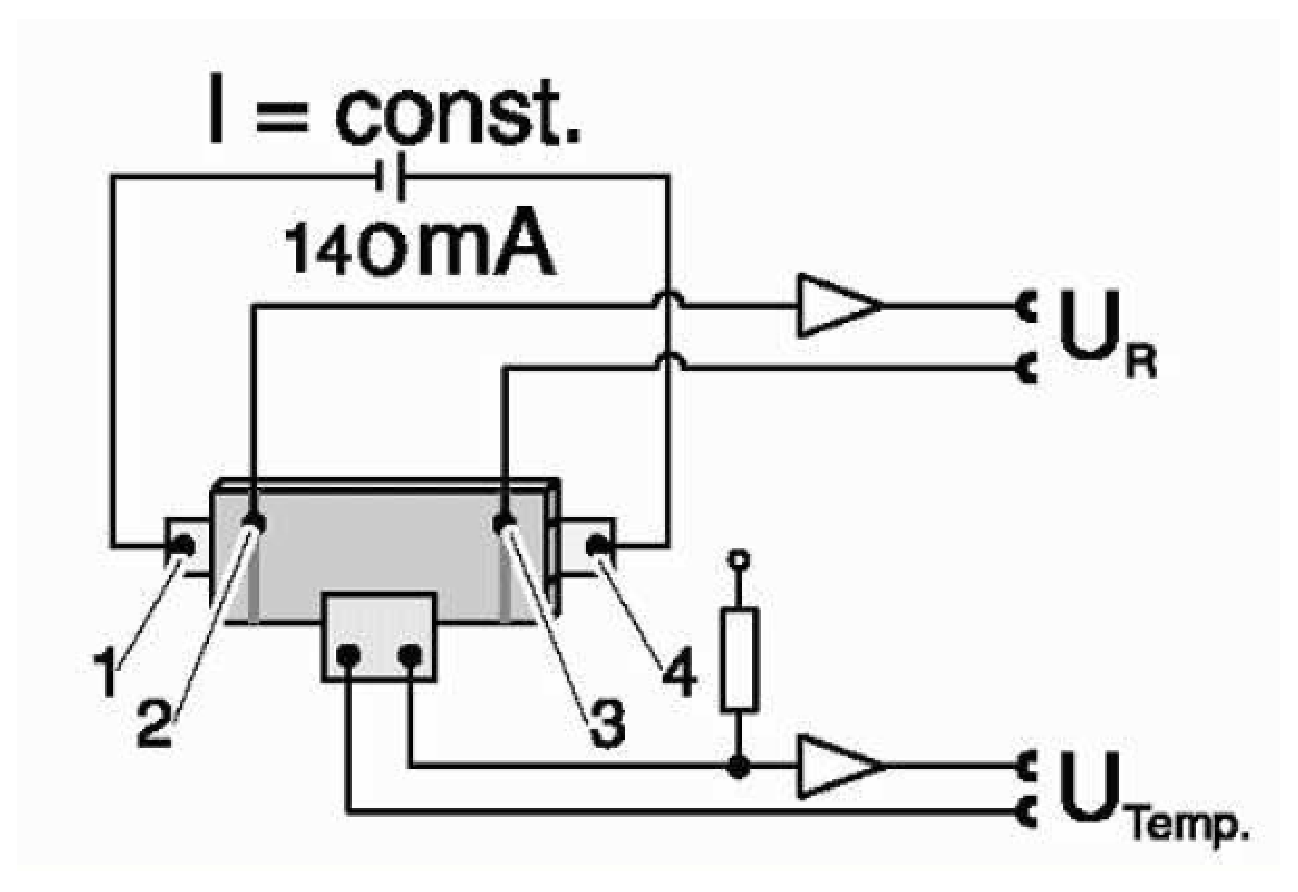
\includegraphics[scale = 0.4]{setup.eps}
\caption{\label{setup} This is the measurement setup.}
\end{figure}

\section{Measurement results}

The resulting plot of the resistance versus temperature can be seen in Figure \ref{res_plot}. In this figure we see that around the temperature $T \approx 96 K$ there is a sharp drop in the resistance. Since this drop is not instantaneous we will define the critical temperature $T_c$ as the mean value of $T$ during the drop, this yields $T_c \approx 94.3$ [K].

\begin{figure}
\centering
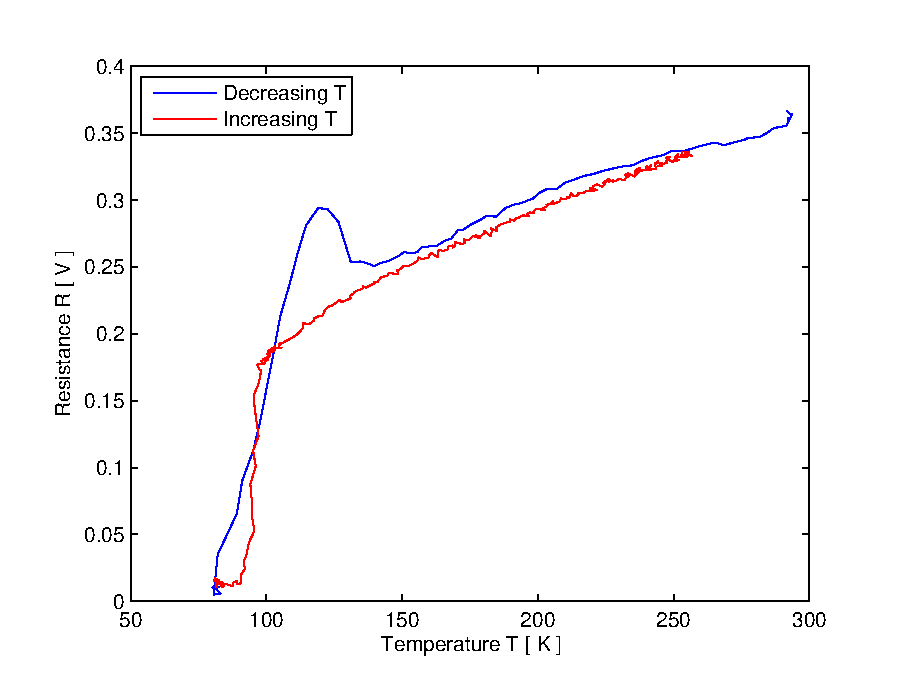
\includegraphics[scale = 0.9]{SC_plot.eps}
\caption{\label{res_plot}Here we can see the electrical resistance, measured in volts, plotted versus the temperature of the sample for both decreasing and increasing temperatures.}
\end{figure}
\
\section{Discussion}

In Figure \ref{res_plot} we see the plot of the electrical resistance versus the sample temperature, we see an odd bump in the cooling curve near $T \approx 120$ [K]. This bump is the result of the measuring module malfunctioning causing liquid nitrogen to leak in, and should therefore be disregarded.

We can also see that the heating-curve does not exactly match the cooling-curve for temperatures above this bump. This difference is likely caused by the fact that the sensor measuring the temperature of the sample is glued on to the surface of the sample. During cooling the sensor will therefore show a temperature slightly lower than the sample temperature of the sample and during heating the sensor will show a slightly higher temperature. So the resistance during cooling shall be higher than what the sensor told us. 

\section{Conclusions}

We have determined that the critical temperature of the YBCO sample is $T_c \approx 94.3$ [K]. From table 2 on page 262 in Kittel (8th edition) we find the critical temperature of $\mathrm{YBa_2Cu_3O_{6.9}}$ listed as $T_c \approx 90$ [K]. The deviation from our experimental value might be due to the uncertainty in amount of oxygen in this specific sample. As we mentioned, the measurement module was malfunctioning so this is also a possible reason to the deviation. 

\end{document}